\documentclass[tikz]{standalone}
\usetikzlibrary{shapes.geometric, arrows,fit,matrix,positioning,shapes.multipart}
\usetikzlibrary{arrows}
\usetikzlibrary{positioning}

\tikzstyle{arrow} = [thick,->,>=stealth]
\begin{document}
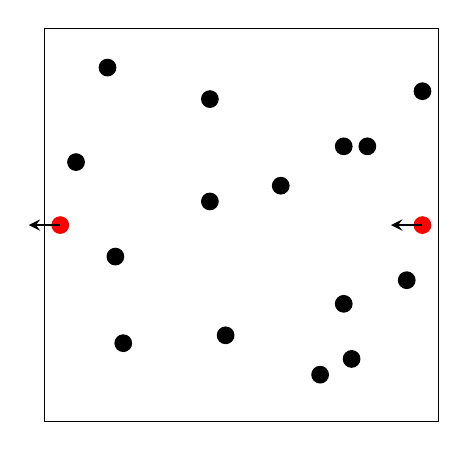
\begin{tikzpicture}
\draw (0,0) rectangle (5,5) ;

\filldraw[color=red] (0.2,2.5) circle (3pt);
\draw [arrow] (0.2,2.5) -- (-0.2,2.5);
\filldraw[color=red] (4.8,2.5) circle (3pt);
\draw [arrow] (4.8,2.5) -- (4.4,2.5);

\filldraw[color=black] (1,1) circle (3pt);
\filldraw[color=black] (2.3,1.1) circle (3pt);
\filldraw[color=black] (3.9,0.8) circle (3pt);
\filldraw[color=black] (4.6,1.8) circle (3pt);
\filldraw[color=black] (0.4,3.3) circle (3pt);
\filldraw[color=black] (2.1,2.8) circle (3pt);
\filldraw[color=black] (3.8,3.5) circle (3pt);
\filldraw[color=black] (4.8,4.2) circle (3pt);
\filldraw[color=black] (0.8,4.5) circle (3pt);
\filldraw[color=black] (2.1,4.1) circle (3pt);
\filldraw[color=black] (3.8,1.5) circle (3pt);
\filldraw[color=black] (3.5,0.6) circle (3pt);
\filldraw[color=black] (3.0,3.0) circle (3pt);   
\filldraw[color=black] (4.1,3.5) circle (3pt);          
\filldraw[color=black] (0.9,2.1) circle (3pt);
\end{tikzpicture}
\end{document}